\secslide{Code Quality}

\begin{darkframe}
  \begin{center}
    \uncover<2>{
      
\includegraphics[width=0.35\textwidth]{graphics/patrick.jpg}
    }
    \\[1.5em]
    \begin{minipage}{0.8\textwidth}
      \begin{minted}{python}
        def f(x,y=0):return[x[i]+y if x[i]>0else y-x[i]for i in range(len(x))]
      \end{minted}
    \end{minipage}
    \\[3em]
    \uncover<2>{
      \huge\textcolor{ccyan}{This runs, but do you trust it?}
    }
  \end{center}

  \begin{tikzpicture}[remember picture, overlay]
    \coordinate (pos) at ([xshift=-2cm, yshift=1cm]current page.south east);
    \node [rotate around={30:(pos)}, align=center] at (pos) {Shamelessly taken from\\Stefan's talk :)};
  \end{tikzpicture}
\end{darkframe}

\begin{darkframe}{Code Quality Terminology}
  \Huge
  \begin{enumerate}
    \setlength{\itemsep}{2em}
    \item \textcolor{ccyan}{Surface Quality}
      \begin{itemize}
        \item [\to] Formatting: Layout, naming conventions, whitespaces
      \end{itemize}
    \item \textcolor{ccyan}{Semantic Quality}
      \begin{itemize}
        \item [\to] Docstrings, type hinting
      \end{itemize}
    \item \textcolor{ccyan}{Testability}
      \begin{itemize}
        \item [\to] Writing (simple) code that is easy to test
      \end{itemize}
  \end{enumerate}
\end{darkframe}

\begin{frame}{Surface Quality: PEP 8}
  \begin{center}
    \huge\iref{https://peps.python.org/pep-0008/}{Python Enhancement Proposal No. 8 (PEP 8)}
  \end{center}
  \begin{itemize}
    \setlength{\itemsep}{1em}
    \item Coding convention comprising the standard library, all about readability
    \item Key Aspects:\\
      \begin{center}
      \begin{tblr}{
          colspec={c c c},
          rows={font=\bfseries\Large, fg=ccyan, rowsep=0.25cm},
          columns={colsep=0.75cm},
        }
        Code Layout & String Quotes & Whitespaces \\
        Trailing Commas & Comments & Naming Conventions
      \end{tblr}
      \end{center}
  \end{itemize}
\end{frame}

\begin{darkframe}[fragile]{Surface Quality: PEP 8}
  \begin{center}
    \begin{tikzpicture}[remember picture]
      \node [anchor=east, outer sep=10pt] (wrong) at ([xshift=-1cm]current page.center) {
      \begin{minipage}{0.3\textwidth}
        \begin{minted}{python}
          def add(a, b): return a+b
          from rich import print
          import os, math
          def printPi():print(math.pi)
        \end{minted}
      \end{minipage}
    };

      \node [anchor=west, outer sep=10pt] (correct) at ([xshift=1cm]current page.center) {
      \begin{minipage}{0.3\textwidth}
        \begin{minted}{python}
          import os, math

          from rich import print


          def add(a, b):
              return a + b


          def print_pi():
              print(math.pi)
        \end{minted}
      \end{minipage}
    };

      \draw [->, >=latex] (wrong) -- (correct);
  \end{tikzpicture}
  \end{center}
\end{darkframe}

\begin{frame}{Surface Quality: Tools}
  \large
  \begin{description}[\iref{https://pycodestyle.pycqa.org/en/latest/}{pycodestyle}]
    \setlength{\itemsep}{1em}
    \item [\iref{https://pycodestyle.pycqa.org/en/latest/}{pycodestyle}] Strict \texttt{PEP8} formatter.
    \item [\iref{https://flake8.pycqa.org/en/latest/}{flake8}] \texttt{pyflakes} + \texttt{pycodestyle} + \texttt{optional plugins}.
    \item [\iref{https://black.readthedocs.io/en/stable/}{black}] Follows \texttt{PEP8} and adds it's
      own strict rules (\eg, 88 chars limit).
    \item [\iref{https://pycqa.github.io/isort/}{isort}] Sorts imports so you don't have to.
    \item [\iref{https://docs.astral.sh/ruff/}{Ruff}] All of the above, highly customizable using
      \texttt{pyproject.toml} or \texttt{ruff.toml}, and extremely fast.
  \end{description}
  \vspace{0.5cm}
  \begin{center}
    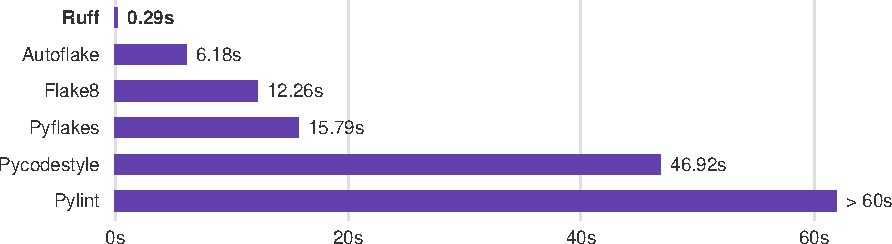
\includegraphics[width=0.7\textwidth]{graphics/speed_ruff.pdf}\src{docs.astral.sh/ruff}
  \end{center}
\end{frame}

\begin{splitframe}[fragile]{Surface Quality: Ruff}{pyproject.toml}
  \begin{columns}[t,onlytextwidth]
    \begin{column}{0.58\textwidth}
      {
      \usemintedstyle{code-light}
      \begin{itemize}
        \setlength{\itemsep}{2.5em}
        \item Install via \texttt{uv} as global tool or add to your project:
          \begin{minted}{shell-session}
            $ uv tool install ruff@latest
            $ uv add --dev ruff
          \end{minted}
        \item Two tools in one: \emph{Formatter} and \emph{linter}
          \begin{minted}{shell-session}
            $ ruff check
            $ ruff format
          \end{minted}
        \item Ruff supports over \emph{800} lint rules, inspired by the popular tools
          shown earlier \to{} See \iref{https://docs.astral.sh/ruff/rules/}{Rules}.
          \begin{itemize}
            \setlength{\itemsep}{1em}
            \item [\to] Configure everything in \texttt{pyproject.toml} or \texttt{ruff.toml}.
            \item [\to] Disable specific rules that you don't need in your project, \eg, \texttt{B905} \textit{zip-without-explicit-strict}.
          \end{itemize}
      \end{itemize}
      }
    \end{column}
    \hfill
    \begin{column}{0.38\textwidth}
      \footnotesize
      \vspace*{0.25cm}
      \begin{minted}{toml}
        [tool.ruff]
        target-version = "py313"
        line-length = 88
        extend-exclude = ["tests"]

        [tool.ruff.lint]
        extend-select = [
          "I",   # isort
          "E",   # pycodestyle
          "F",   # Pyflakes
          "UP",  # pyupgrade
          "B",   # flake8-bugbear
          "SIM", # flake8-simplify
        ]
        ignore = ["B905"]

        fixable = ["ALL"]
        unfixable = []

        [tool.ruff.lint.per-file-ignores]
        "examples/**" = ["I"]

        [tool.ruff.format]
        quote-style = "double"
        indent-style = "space"
        line-ending = "auto"
        skip-magic-trailing-comma = false
        docstring-code-format = true

        [tool.ruff.lint.isort]
        known-first-party = ["my_package"]
      \end{minted}
    \end{column}
  \end{columns}
\end{splitframe}

\begin{splitframe}[fragile]{Semantic Quality: Docstrings}{NumPy Style}
  \begin{columns}[t,onlytextwidth]
    \begin{column}{0.58\textwidth}
      {
      \usemintedstyle{code-light}
      \begin{itemize}
        \setlength{\itemsep}{2.5em}
        \item Explains what your code does.
        \item Can be understood by IDEs and autocompletion tools
        \item Necessary for well-written docs (later)
        \item Structure:
          \begin{itemize}
            \item [\to] Triple double quotes (\mintinline{python}+"""..."""+)
            \item Human-readable, complete sentences describing your code
            \item Explanation of parameters, returns, and exceptions
          \end{itemize}
        \item Many different styles available: Use \emph{one} and \emph{stick to it}.
      \end{itemize}
      }
    \end{column}
    \hfill
    \begin{column}{0.38\textwidth}
      \footnotesize
      \vspace*{0.25cm}
      \begin{minted}{python}
        def draw_sampling_opts(size: int) -> Dict:
            """Draws randomized sampling parameters
            for the simulation.

            Parameters
            ----------
            size : int
                Number of parameters to draw, equal
                to number of images.

            Returns
            -------
            samp_opts : dict
                Sampling options/parameters stored
                inside a dictionary.
            """
      \end{minted}
    \end{column}
  \end{columns}
\end{splitframe}

{
\usemintedstyle{code-light}
\begin{frame}[fragile]{Semantic Quality: Type Hinting}
  \begin{center}
    \huge\textcolor{ccyan}{Python is dynamically typed, but\dots}
  \end{center}
  \begin{itemize}
    \setlength{\itemsep}{1em}
    \item \dots you can still declare types for variables:
      \begin{minted}{python}
        foo: int = 1
        bar: str = "app"
        baz: np.ndarray = np.array([...])

        def func(a: int, b: int=42) -> int:
          return a + b
      \end{minted}
    \item [\to] Improved code readability
    \item IDE and linting support, \eg, through code completion
    \item But: Type hinting is \emph{not} enforced at runtime and one has
      to consider dynamic types

    \item Tools:
      \begin{description}[\iref{https://microsoft.github.io/pyright/}{pyright}]
        \item [\iref{https://mypy-lang.org/}{mypy}] Good for CI/CLI
        \item [\iref{https://microsoft.github.io/pyright/}{pyright}] Proprietary tool, but faster and with VSCode integration
      \end{description}
  \end{itemize}
\end{frame}
}

\begin{splitframe}[fragile]{Automation: pre-commit Hook}{.pre-commit-config.yaml}{0.5}
  \begin{columns}[t,onlytextwidth]
    \begin{column}{0.48\textwidth}
      {
      \usemintedstyle{code-light}
      \begin{itemize}
        \setlength{\itemsep}{2em}
        \item \iref{https://pre-commit.com/}{pre-commit} does all the formatting and linting for you
        \item Install via \texttt{uv}:
          \begin{minted}{shell-session}
            $ uv pip install pre-commit
          \end{minted}
        \item Many different hooks available:
          \begin{itemize}
            \item \texttt{ruff}, \texttt{mypy}, \iref{https://github.com/codespell-project/codespell}{codespell}, and many more\dots
          \end{itemize}
        \item Runs all tools defined in \texttt{.pre-commit-config.yaml}
        \item Run \mintinline{shell-session}+$ pre-commit install+ to install
          hooks in your project
        \item \mintinline{shell-session}{pre-commit} runs automatically whenever something is comitted
          using \mintinline{shell-session}{$ git commit ...}
      \end{itemize}
      }
    \end{column}
    \hfill
    \begin{column}{0.48\textwidth}
      \footnotesize
      \vspace*{0.25cm}
      \begin{minted}{yaml}
        repos:
          - repo: https://github.com/pre-commit/pre-commit-hooks
            rev: "v5.0.0"  # <- git version tag
            hooks:
              - id: check-added-large-files
              - id: check-case-conflict
              - id: check-merge-conflict
              - id: check-symlinks
              - id: check-yaml
              - id: debug-statements
              - id: end-of-file-fixer
              - id: mixed-line-ending
              - id: name-tests-test
                args: ["--pytest-test-first"]
              - id: requirements-txt-fixer
              - id: trailing-whitespace

          - repo: https://github.com/astral-sh/ruff-pre-commit
            rev: "v0.12.3"
            hooks:
              - id: ruff-format
              - id: ruff-check
                args: ["--fix", "--show-fixes"]

          - repo: https://github.com/codespell-project/codespell
            rev: v2.4.1
            hooks:
            - id: codespell
              additional_dependencies:
                - tomli
      \end{minted}
    \end{column}
  \end{columns}
\end{splitframe}

\begin{frame}{Further Reading: Code Quality}
  \begin{itemize}
    \setlength{\itemsep}{1em}
    \item \iref{https://indico.desy.de/event/43817/sessions/19711/attachments/97900/134904/Code\%20Quality\%20PYOPP.pdf}{Stefans Talk On Code Quality}
    \item \iref{https://peps.python.org/pep-0008/}{Python Enhancement Proposal No. 8 (PEP 8)}
    \item \iref{https://docs.astral.sh/ruff/}{Ruff Docs}
    \item \iref{https://mypy.readthedocs.io/en/stable/}{mypy Docs}
    \item \iref{https://microsoft.github.io/pyright/}{pyright Docs}
    \item \iref{https://pre-commit.com/}{pre-commit}
    \item \iref{https://github.com/pre-commit/pre-commit-hooks}{pre-commit-hooks}
    \item \iref{https://github.com/codespell-project/codespell}{codespell}
  \end{itemize}
\end{frame}
